\documentclass[11pt,a4paper,]{article}
\usepackage{lmodern}

\usepackage{amssymb,amsmath}
\usepackage{ifxetex,ifluatex}
\usepackage{fixltx2e} % provides \textsubscript
\ifnum 0\ifxetex 1\fi\ifluatex 1\fi=0 % if pdftex
  \usepackage[T1]{fontenc}
  \usepackage[utf8]{inputenc}
\else % if luatex or xelatex
  \usepackage{unicode-math}
  \defaultfontfeatures{Ligatures=TeX,Scale=MatchLowercase}
\fi
% use upquote if available, for straight quotes in verbatim environments
\IfFileExists{upquote.sty}{\usepackage{upquote}}{}
% use microtype if available
\IfFileExists{microtype.sty}{%
\usepackage[]{microtype}
\UseMicrotypeSet[protrusion]{basicmath} % disable protrusion for tt fonts
}{}
\PassOptionsToPackage{hyphens}{url} % url is loaded by hyperref
\usepackage[unicode=true]{hyperref}
\hypersetup{
            pdftitle={Report on Happiness up to 2022},
            pdfborder={0 0 0},
            breaklinks=true}
\urlstyle{same}  % don't use monospace font for urls
\usepackage{geometry}
\geometry{a4paper, centering, text={16cm,25cm}}
\usepackage[style=authoryear-comp,]{biblatex}
\addbibresource{references.bib}
\usepackage{longtable,booktabs}
% Fix footnotes in tables (requires footnote package)
\IfFileExists{footnote.sty}{\usepackage{footnote}\makesavenoteenv{long table}}{}
\usepackage{graphicx,grffile}
\makeatletter
\def\maxwidth{\ifdim\Gin@nat@width>\linewidth\linewidth\else\Gin@nat@width\fi}
\def\maxheight{\ifdim\Gin@nat@height>\textheight\textheight\else\Gin@nat@height\fi}
\makeatother
% Scale images if necessary, so that they will not overflow the page
% margins by default, and it is still possible to overwrite the defaults
% using explicit options in \includegraphics[width, height, ...]{}
\setkeys{Gin}{width=\maxwidth,height=\maxheight,keepaspectratio}
\IfFileExists{parskip.sty}{%
\usepackage{parskip}
}{% else
\setlength{\parindent}{0pt}
\setlength{\parskip}{6pt plus 2pt minus 1pt}
}
\setlength{\emergencystretch}{3em}  % prevent overfull lines
\providecommand{\tightlist}{%
  \setlength{\itemsep}{0pt}\setlength{\parskip}{0pt}}
\setcounter{secnumdepth}{5}

% set default figure placement to htbp
\makeatletter
\def\fps@figure{htbp}
\makeatother


\title{Report on Happiness up to 2022}

%% MONASH STUFF

%% CAPTIONS
\RequirePackage{caption}
\DeclareCaptionStyle{italic}[justification=centering]
 {labelfont={bf},textfont={it},labelsep=colon}
\captionsetup[figure]{style=italic,format=hang,singlelinecheck=true}
\captionsetup[table]{style=italic,format=hang,singlelinecheck=true}


%% FONT
\RequirePackage{bera}
\RequirePackage[charter,expert,sfscaled]{mathdesign}
\RequirePackage{fontawesome}

%% HEADERS AND FOOTERS
\RequirePackage{fancyhdr}
\pagestyle{fancy}
\rfoot{\Large\sffamily\raisebox{-0.1cm}{\textbf{\thepage}}}
\makeatletter
\lhead{\textsf{\expandafter{\@title}}}
\makeatother
\rhead{}
\cfoot{}
\setlength{\headheight}{15pt}
\renewcommand{\headrulewidth}{0.4pt}
\renewcommand{\footrulewidth}{0.4pt}
\fancypagestyle{plain}{%
\fancyhf{} % clear all header and footer fields
\fancyfoot[C]{\sffamily\thepage} % except the center
\renewcommand{\headrulewidth}{0pt}
\renewcommand{\footrulewidth}{0pt}}

%% MATHS
\RequirePackage{bm,amsmath}
\allowdisplaybreaks

%% GRAPHICS
\RequirePackage{graphicx}
\setcounter{topnumber}{2}
\setcounter{bottomnumber}{2}
\setcounter{totalnumber}{4}
\renewcommand{\topfraction}{0.85}
\renewcommand{\bottomfraction}{0.85}
\renewcommand{\textfraction}{0.15}
\renewcommand{\floatpagefraction}{0.8}


%\RequirePackage[section]{placeins}

%% SECTION TITLES


%% SECTION TITLES
\RequirePackage[compact,sf,bf]{titlesec}
\titleformat*{\section}{\Large\sf\bfseries\color[rgb]{0.7,0,0}}
\titleformat*{\subsection}{\large\sf\bfseries\color[rgb]{0.7,0,0}}
\titleformat*{\subsubsection}{\sf\bfseries\color[rgb]{0.7,0,0}}
\titlespacing{\section}{0pt}{2ex}{.5ex}
\titlespacing{\subsection}{0pt}{1.5ex}{0ex}
\titlespacing{\subsubsection}{0pt}{.5ex}{0ex}


%% TITLE PAGE
\def\Date{\number\day}
\def\Month{\ifcase\month\or
 January\or February\or March\or April\or May\or June\or
 July\or August\or September\or October\or November\or December\fi}
\def\Year{\number\year}

%% LINE AND PAGE BREAKING
\sloppy
\clubpenalty = 10000
\widowpenalty = 10000
\brokenpenalty = 10000
\RequirePackage{microtype}

%% PARAGRAPH BREAKS
\setlength{\parskip}{1.4ex}
\setlength{\parindent}{0em}

%% HYPERLINKS
\RequirePackage{xcolor} % Needed for links
\definecolor{darkblue}{rgb}{0,0,.6}
\RequirePackage{url}

\makeatletter
\@ifpackageloaded{hyperref}{}{\RequirePackage{hyperref}}
\makeatother
\hypersetup{
     citecolor=0 0 0,
     breaklinks=true,
     bookmarksopen=true,
     bookmarksnumbered=true,
     linkcolor=darkblue,
     urlcolor=blue,
     citecolor=darkblue,
     colorlinks=true}

\usepackage[showonlyrefs]{mathtools}
\usepackage[no-weekday]{eukdate}

%% BIBLIOGRAPHY

\makeatletter
\@ifpackageloaded{biblatex}{}{\usepackage[style=authoryear-comp, backend=biber, natbib=true]{biblatex}}
\makeatother
\ExecuteBibliographyOptions{bibencoding=utf8,minnames=1,maxnames=3, maxbibnames=99,dashed=false,terseinits=true,giveninits=true,uniquename=false,uniquelist=false,doi=false, isbn=false,url=true,sortcites=false}

\DeclareFieldFormat{url}{\texttt{\url{#1}}}
\DeclareFieldFormat[article]{pages}{#1}
\DeclareFieldFormat[inproceedings]{pages}{\lowercase{pp.}#1}
\DeclareFieldFormat[incollection]{pages}{\lowercase{pp.}#1}
\DeclareFieldFormat[article]{volume}{\mkbibbold{#1}}
\DeclareFieldFormat[article]{number}{\mkbibparens{#1}}
\DeclareFieldFormat[article]{title}{\MakeCapital{#1}}
\DeclareFieldFormat[article]{url}{}
%\DeclareFieldFormat[book]{url}{}
%\DeclareFieldFormat[inbook]{url}{}
%\DeclareFieldFormat[incollection]{url}{}
%\DeclareFieldFormat[inproceedings]{url}{}
\DeclareFieldFormat[inproceedings]{title}{#1}
\DeclareFieldFormat{shorthandwidth}{#1}
%\DeclareFieldFormat{extrayear}{}
% No dot before number of articles
\usepackage{xpatch}
\xpatchbibmacro{volume+number+eid}{\setunit*{\adddot}}{}{}{}
% Remove In: for an article.
\renewbibmacro{in:}{%
  \ifentrytype{article}{}{%
  \printtext{\bibstring{in}\intitlepunct}}}

\AtEveryBibitem{\clearfield{month}}
\AtEveryCitekey{\clearfield{month}}

\makeatletter
\DeclareDelimFormat[cbx@textcite]{nameyeardelim}{\addspace}
\makeatother

\author{\sf{\Large\textbf{Zhixiang Yang}\\\large EBS Honours Student\\[0.5cm]}{\Large\textbf{Yiqi Wang}\\\large Master of BA Student\\[0.5cm]}{\Large\textbf{Xintong You}\\\large Master of BA Student\\[0.5cm]}}

\date{\sf\Date~\Month~\Year}
\makeatletter
\lfoot{\sf Yang, Wang, You: \@date}
\makeatother


%%%% PAGE STYLE FOR FRONT PAGE OF REPORTS

\makeatletter
\def\organization#1{\gdef\@organization{#1}}
\def\telephone#1{\gdef\@telephone{#1}}
\def\email#1{\gdef\@email{#1}}
\makeatother
  \organization{Group 07 ETC5513}

  \def\name{Department of\newline Econometrics \&\newline Business Statistics}

  \telephone{(03) 9905 2478}

  \email{BusEco-Econometrics@monash.edu}

\def\webaddress{\url{http://buseco.monash.edu/ebs/consulting/}}
\def\abn{12 377 614 012}
\def\extraspace{\vspace*{1.6cm}}
\makeatletter
\def\contactdetails{\faicon{phone} & \@telephone \\
                    \faicon{envelope} & \@email}
\makeatother

\usepackage[absolute,overlay]{textpos}
\setlength{\TPHorizModule}{1cm}
\setlength{\TPVertModule}{1cm}

%%%% FRONT PAGE OF REPORTS

\def\reporttype{Report for}

\long\def\front#1#2#3{
\newpage
\begin{textblock}{7}(12.7,28.2)\hfill

\includegraphics[height=0.6cm]{AACSB}~~~

\includegraphics[height=0.6cm]{EQUIS}~~~

\includegraphics[height=0.6cm]{AMBA}
\end{textblock}
\begin{singlespacing}
\thispagestyle{empty}
\vspace*{-1.4cm}
\hspace*{-1.4cm}
\hbox to 16cm{
  \hbox to 6.5cm{\vbox to 14cm{\vbox to 25cm{
    
\includegraphics[width=6cm]{monash2}
    \vfill
    
\includegraphics[width=3.5cm]{MBSportrait}
    \vspace{0.4cm}
    \par
    \parbox{6.3cm}{\raggedright
      \sf\color[rgb]{0.00,0.00,0.70}
      {\large\textbf{\name}}\par
      \vspace{.7cm}
      \tabcolsep=0.12cm\sf\small
      \begin{tabular}{@{}ll@{}}\contactdetails
      \end{tabular}
      \vspace*{0.3cm}\par
      ABN: \abn\par
    }
  }\vss}\hss}
  \hspace*{0.2cm}
  \hbox to 1cm{\vbox to 14cm{\rule{1pt}{26.8cm}\vss}\hss\hfill}
  \hbox to 10cm{\vbox to 14cm{\vbox to 25cm{
      \vspace*{3cm}\sf\raggedright
      \parbox{11cm}{\sf\raggedright\baselineskip=1.2cm
         \fontsize{24.88}{30}\color[rgb]{0.70,0.00,0.00}\sf\textbf{#1}}
      \par
      \vfill
      \large
      \vbox{\parskip=0.8cm #2}\par
      \vspace*{2cm}\par
      \reporttype\\[0.3cm]
      \hbox{#3}%\\[2cm]\
      \vspace*{1cm}
      {\large\sf\textbf{\Date~\Month~\Year}}
   }\vss}
  }}
\end{singlespacing}
\newpage
}

\makeatletter
\def\titlepage{\front{\expandafter{\@title}}{\@author}{\@organization}}
\makeatother

\usepackage{setspace}
\setstretch{1.5}

%% Any special functions or other packages can be loaded here.
\usepackage{booktabs}
\usepackage{longtable}
\usepackage{array}
\usepackage{multirow}
\usepackage{wrapfig}
\usepackage{float}
\usepackage{colortbl}
\usepackage{pdflscape}
\usepackage{tabu}
\usepackage{threeparttable}
\usepackage{threeparttablex}
\usepackage[normalem]{ulem}
\usepackage{makecell}
\usepackage{xcolor}


\begin{document}
\titlepage

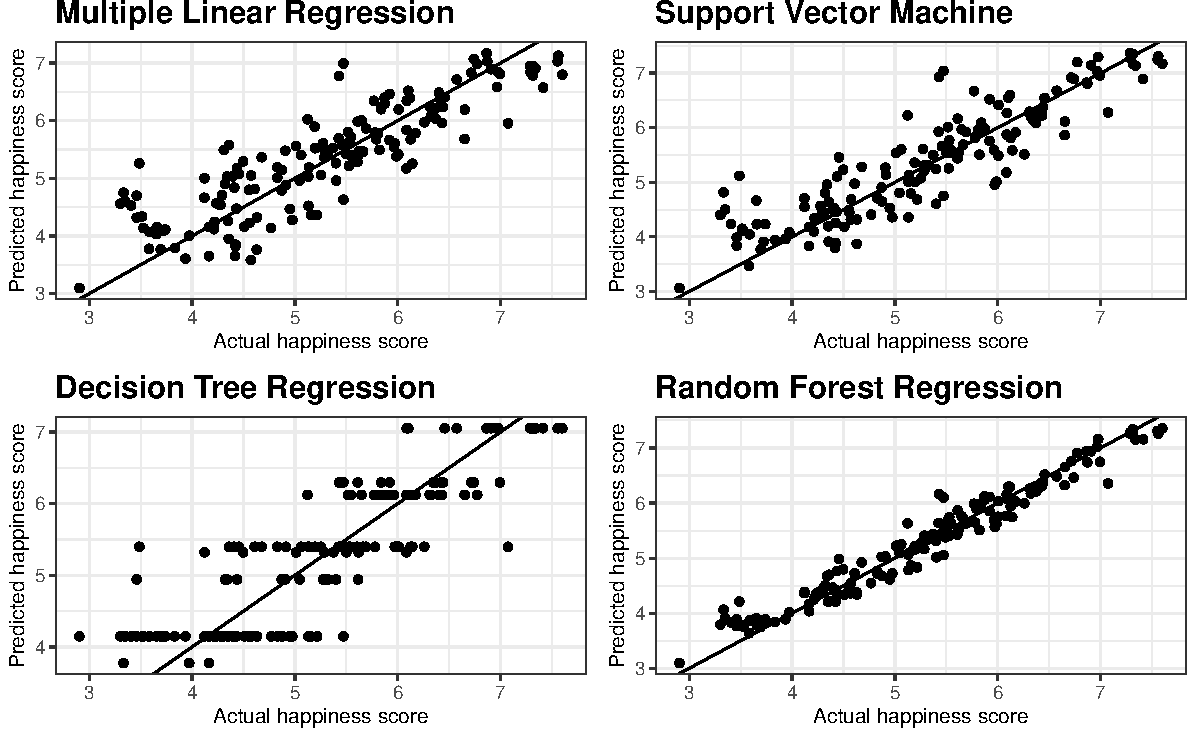
\includegraphics{Assignment4_files/figure-latex/unnamed-chunk-6-1.pdf} 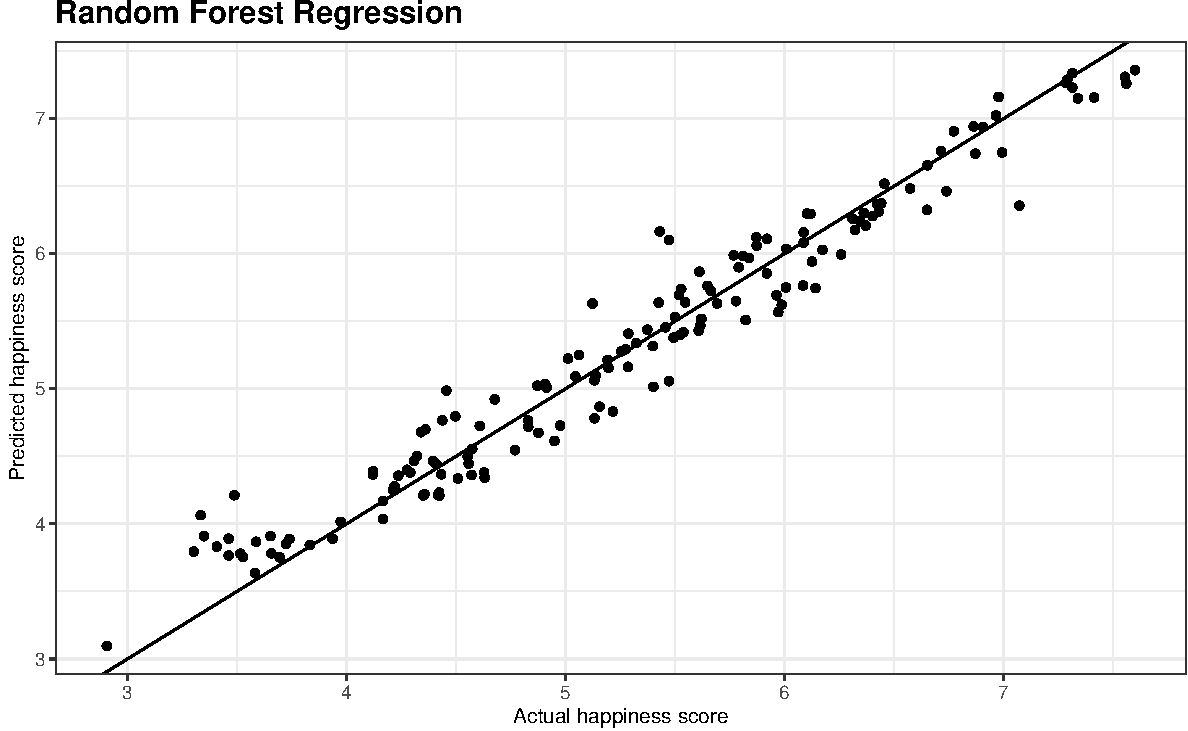
\includegraphics{Assignment4_files/figure-latex/unnamed-chunk-6-2.pdf} 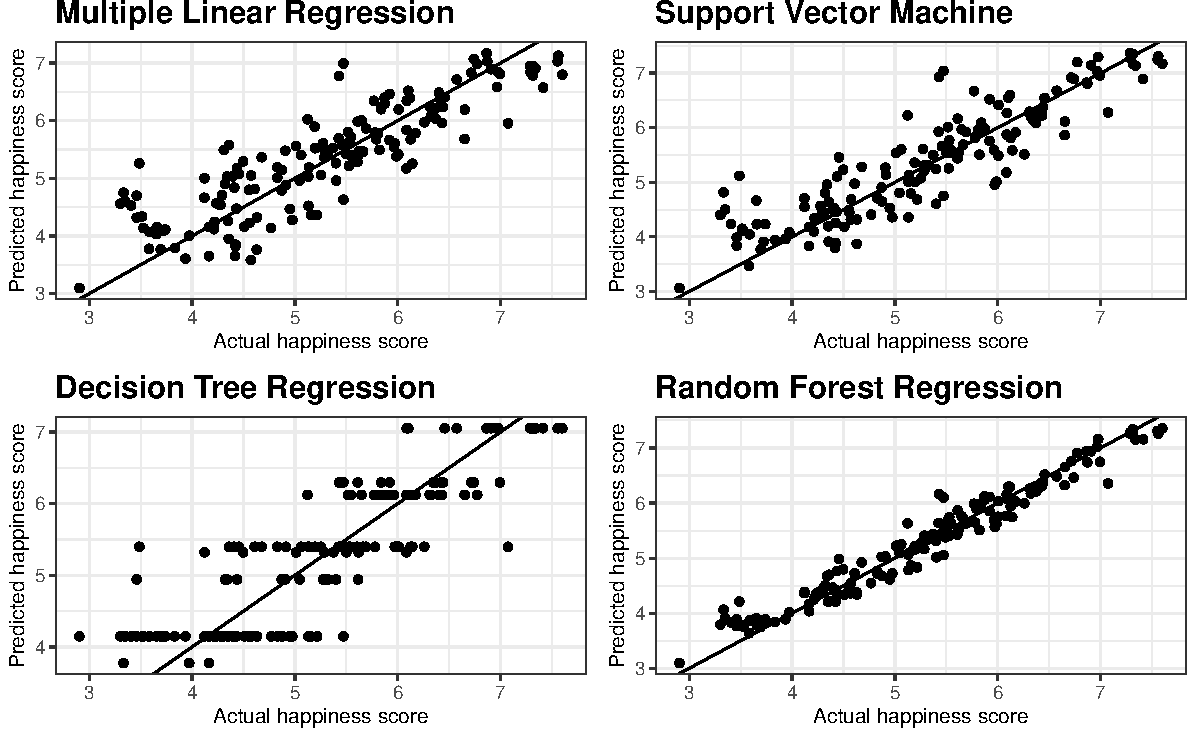
\includegraphics{Assignment4_files/figure-latex/unnamed-chunk-6-3.pdf}

\hypertarget{tree-plot}{%
\section{Tree plot}\label{tree-plot}}

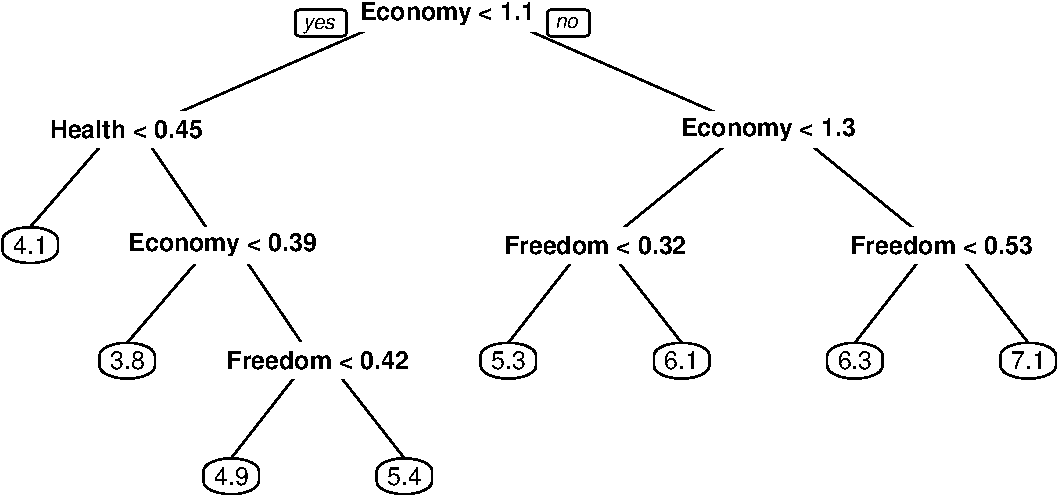
\includegraphics{Assignment4_files/figure-latex/unnamed-chunk-7-1.pdf}

\hypertarget{random-forest-regression}{%
\section{Random Forest regression}\label{random-forest-regression}}

RF model is used to predict causes for Random Forest is a practical way and regularly used in machine learning models. Random Forest Model have the variable selecting system (via bootstrapping) to decide the most significant tree and can reduce overwriting compared with decision tree.With that said, random forests are a strong modeling technique and much more robust comparing with many different methods. (Liberman, 2017). We can see from the plot that this model have captured the data well in the past few years.

From the report, we can see that our model is for 2020 data.

\[
\begin{aligned}
log(score)= -4.6000-0.0008\ cpi+0.2591\ log(economy)\\-0.0026\ log(population)+0.0114\ log(health)+0.0032log(year)
\end{aligned}
\]

We can see that the total proportion of variance explained by the model with these variables are 60.49\%. For the 4 predictors, the economy status(GDP per capita) contribute most to the happiness scores than other variables.

\hypertarget{factor-importance}{%
\section{Factor importance}\label{factor-importance}}

Here, we concluded that the best method to fit the 2022 data is the Random Forest. This model will also allow us to tell the importance of variables via a factor loading summary table.

\begin{table}

\caption{\label{tab:unnamed-chunk-8}Variable importance for Random Forest model}
\centering
\begin{tabular}[t]{l|r}
\hline
  & IncNodePurity\\
\hline
\cellcolor{gray!6}{Economy} & \cellcolor{gray!6}{348.66900}\\
\hline
Health & 327.08463\\
\hline
\cellcolor{gray!6}{Freedom} & \cellcolor{gray!6}{169.32991}\\
\hline
Generosity & 97.79738\\
\hline
\end{tabular}
\end{table}

In this table, we can conclude that the most important variables on explaining the happiness scores will be the Happiness and Health.

\hypertarget{we-abandon-the-current-dataset-to-add-more-variables}{%
\section{We abandon the current dataset to add more variables}\label{we-abandon-the-current-dataset-to-add-more-variables}}

\begin{verbatim}
## 
## Call:
## lm(formula = `Happiness Score` ~ Health + Economy + Freedom + 
##     Generosity, data = dataall)
## 
## Residuals:
##      Min       1Q   Median       3Q      Max 
## -1.88683 -0.36864  0.04779  0.39916  1.76462 
## 
## Coefficients:
##             Estimate Std. Error t value Pr(>|t|)    
## (Intercept)  2.43744    0.07530  32.370  < 2e-16 ***
## Health       1.22320    0.13921   8.787  < 2e-16 ***
## Economy      1.45432    0.08415  17.282  < 2e-16 ***
## Freedom      1.37218    0.10958  12.522  < 2e-16 ***
## Generosity   1.17021    0.13967   8.379 2.52e-16 ***
## ---
## Signif. codes:  0 '***' 0.001 '**' 0.01 '*' 0.05 '.' 0.1 ' ' 1
## 
## Residual standard error: 0.582 on 772 degrees of freedom
## Multiple R-squared:  0.732,  Adjusted R-squared:  0.7307 
## F-statistic: 527.3 on 4 and 772 DF,  p-value: < 2.2e-16
\end{verbatim}

\begin{table}

\caption{\label{tab:unnamed-chunk-9}Linear regression model for happiness scores without new data}
\centering
\begin{tabular}[t]{l|r|r|r|r}
\hline
  & Estimate & Std. Error & t value & Pr(>|t|)\\
\hline
\cellcolor{gray!6}{(Intercept)} & \cellcolor{gray!6}{2.437442} & \cellcolor{gray!6}{0.0752984} & \cellcolor{gray!6}{32.370444} & \cellcolor{gray!6}{0}\\
\hline
Health & 1.223204 & 0.1392052 & 8.787054 & 0\\
\hline
\cellcolor{gray!6}{Economy} & \cellcolor{gray!6}{1.454316} & \cellcolor{gray!6}{0.0841520} & \cellcolor{gray!6}{17.282015} & \cellcolor{gray!6}{0}\\
\hline
Freedom & 1.372180 & 0.1095802 & 12.522156 & 0\\
\hline
\cellcolor{gray!6}{Generosity} & \cellcolor{gray!6}{1.170207} & \cellcolor{gray!6}{0.1396671} & \cellcolor{gray!6}{8.378545} & \cellcolor{gray!6}{0}\\
\hline
\end{tabular}
\end{table}

\hypertarget{what-is-the-correlation-between-these-variables-in-linear-model.}{%
\section{What is the correlation between these variables in linear model.}\label{what-is-the-correlation-between-these-variables-in-linear-model.}}

One advantage of multivariate linear regression is that it can allow us to analyse the relationship between different variables in a statistical coherent way. We can start with the correlation between each variables.

In order to better analyse the relationships, I add two new variables, which are CPI values and the population size for each country. However, due to the limitation of the new dataset, we can only conduct our analysis based on the 2020 data.

\begin{verbatim}
## 
## Call:
## lm(formula = log_score ~ cpi + log_eco + log_population + log_health + 
##     year, data = lognarm_hapall)
## 
## Coefficients:
##    (Intercept)             cpi         log_eco  log_population      log_health  
##     -4.5998547      -0.0007945       0.2590779      -0.0025806       0.0113946  
##           year  
##      0.0031566
\end{verbatim}

\hypertarget{the-countries-that-we-missed-in-the-dataset.}{%
\section{The countries that we missed in the dataset.}\label{the-countries-that-we-missed-in-the-dataset.}}

\begin{verbatim}
## 641 codes from your data successfully matched countries in the map
## 1 codes from your data failed to match with a country code in the map
## 109 codes from the map weren't represented in your data
\end{verbatim}

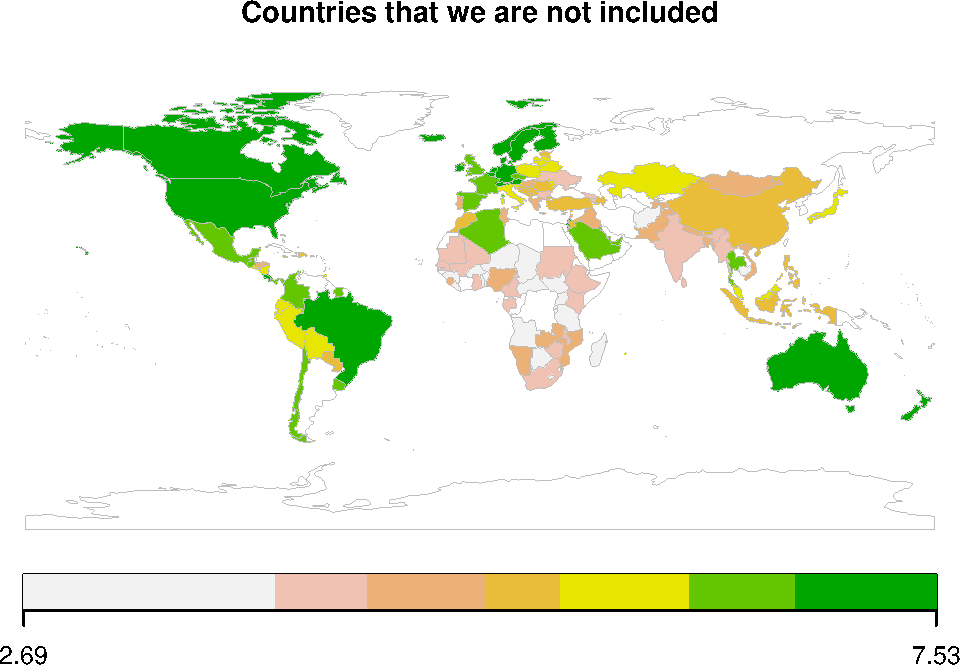
\includegraphics{Assignment4_files/figure-latex/unnamed-chunk-11-1.pdf}

\hypertarget{residual-diagonistic}{%
\section{Residual Diagonistic}\label{residual-diagonistic}}

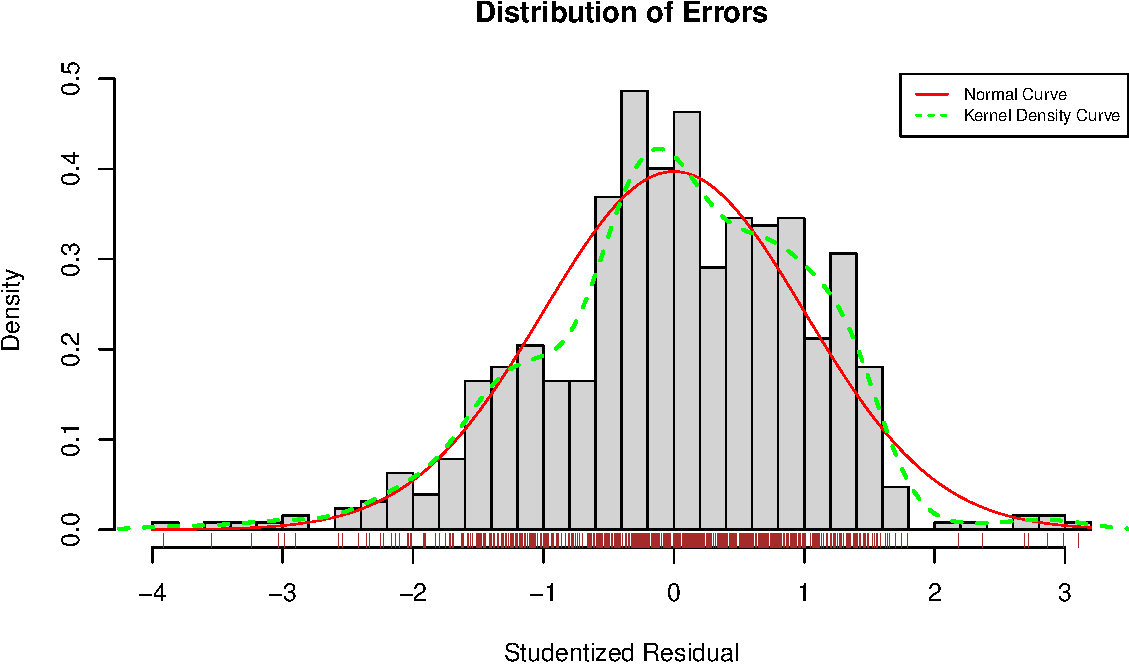
\includegraphics{Assignment4_files/figure-latex/unnamed-chunk-12-1.pdf}

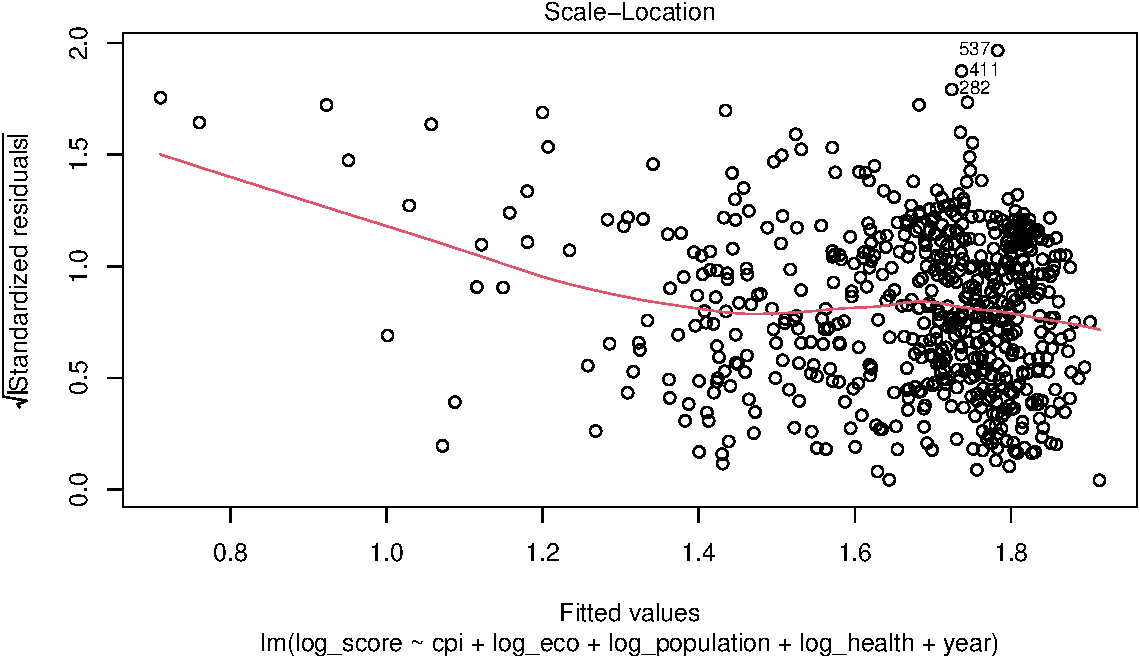
\includegraphics{Assignment4_files/figure-latex/unnamed-chunk-13-1.pdf}

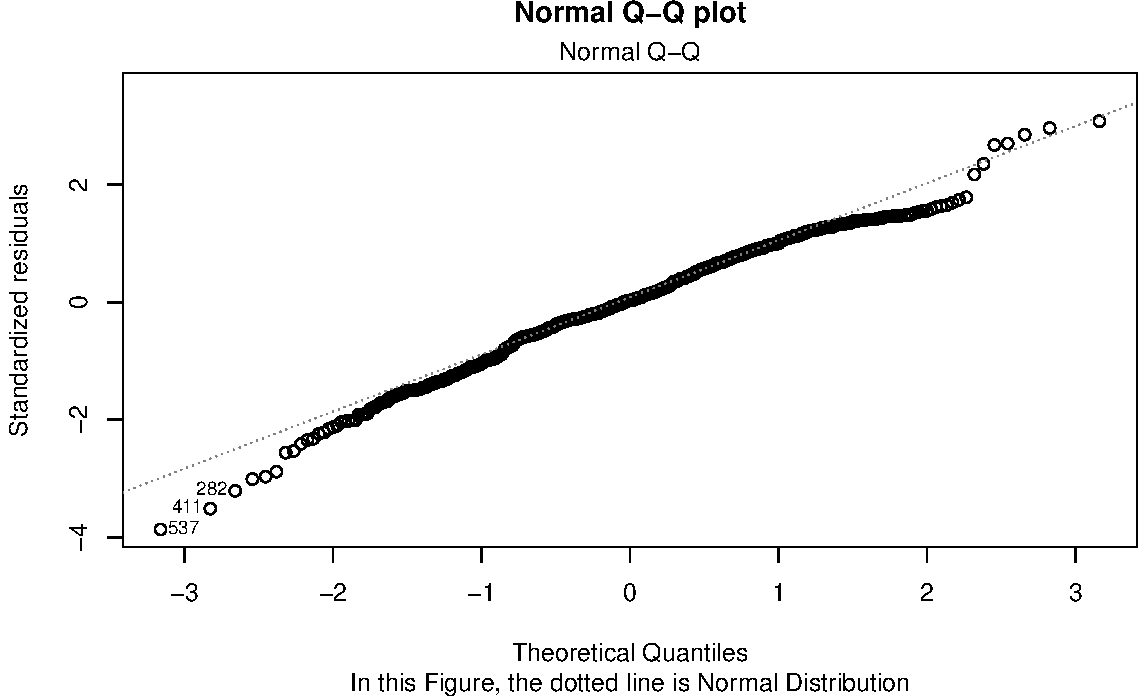
\includegraphics{Assignment4_files/figure-latex/unnamed-chunk-14-1.pdf}

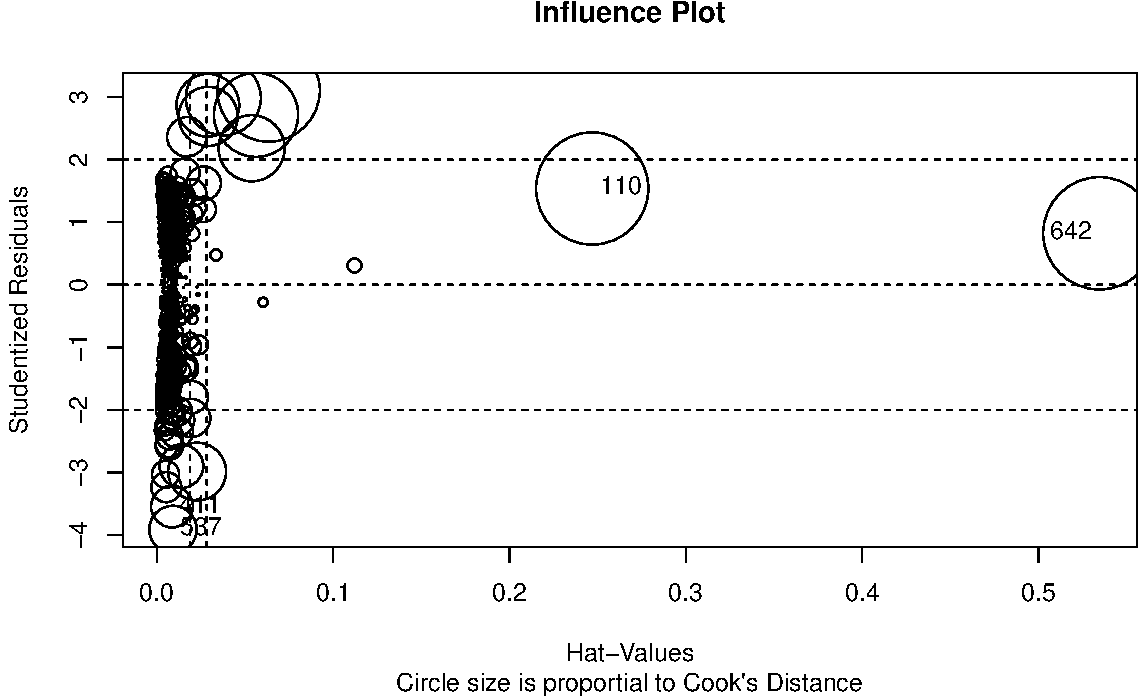
\includegraphics{Assignment4_files/figure-latex/unnamed-chunk-15-1.pdf}

\begin{verbatim}
##        StudRes         Hat      CookD
## 110  1.5379757 0.246899853 0.12896655
## 411 -3.5457416 0.008605488 0.01786073
## 537 -3.9107652 0.009146505 0.02300857
## 642  0.8219777 0.534532896 0.12938311
\end{verbatim}

\printbibliography

\end{document}
